\chapter{Multilayer characterization}\label{multilayercharacterization}
\begin{figure}
	\centering
\def\svgwidth{\textwidth}
\input{ERDA.pdf_tex}
\caption{An example of results as obtained by ERDA. The different elements that are present in the sample are observed as "banana peaks", the curved signals that are visible in the graph. The present iodine is the result of backscattered ions from the target beam, there is no iodine present in the measured sample.}
\label{ERDA}
\end{figure}
\section{Elastic Recoil Detection Analysis}
The elemental composition of the multilayers in this work have been determined using Elastic Recoil Detection Analysis (ERDA). In this work, the Tandem Laboratory at Uppsala University has been used to perform these ERDA measurements. The setup at used at the Tandem Laboratory is described in more detail elsewhere \cite{ERDA_UU}. The name of this technique come from the basic principles of ERDA, a beam of high energetic ions are targeted at a sample after which elastic scattering occurs, upon this scattering interaction some of the atoms in the sample are ejected (or recoiled) \cite{ERDA_0}. The recoiled atoms are measured using an energy-dependent detector. Using the atomic number of the target elements and the energy of the recoiled atoms, compositional information can be obtained. Such an obtained ERDA spectrum can be observed in Figure \ref{ERDA}. Upon collision, light elements are most likely to be ejected in the forward direction. This technique is less suitable for heavier elements as they do not recoil as easily and overlap with backscattered ions \cite{thesis_naureen}. The energy of the beam depends on what sample is characterized, but can be in range from a few MeV to 200 MeV \cite{ERDA_1}. In this work, a primary $^{\text{127}}$I$^{\text{8+}}$ beam with an energy of 36 MeV has been used at an incident angle of 67.5° relative to the surface normal, the energy detector was placed at a recoil scattering angle of 45°. The measured spectrum has been analysed using the Potku software \cite{potku} in order to determine the elemental composition of the sample. 
\section{X-ray Photoelectron Spectroscopy}
X-Ray Photoelectron Spectroscopy (XPS) has been used in this work to analyse the bonding of the boron and carbon atoms that are present in the film. XPS provides qualitative and quantitative information about the chemical composition, and chemical bonds in the sample near the probed surface. The basic principle behind this technique is based on the photoelectric effect, which describes the emission of electrons when a material is irradiated by photons \cite{Einstein}. During an XPS measurement, a sample is irradiated by X-Rays with a known photon energy, leading to electrons being emitted due to the photoelectric effect. During the experiment, the total kinetic energy of the ejected electrons is being measured. The binding energy $E_\text{b}$ is related to this kinetic energy as:
\begin{equation}\label{XPSequation}
	E_\text{b} = h\nu - (E_\text{k} + \phi).
\end{equation}
Where term $h\nu$ is simply the Planck constant multiplied by the frequency of the incident photons, representing the energy of the incident X-rays. The expression $\phi$ is the work function of the instrument, which appears due to the practical situation that the sample is in electrical contact with the spectrometer, in a basic sense the work function  represents the minimum energy that is needed to remove an electron from the instrument \cite{XPS_book}. Since each element has its unique set of binding energies, equation \ref{XPSequation} can be used to see which elements were present in the sample. What makes this particular powerful is that the binding energy of an element is affected by the chemical surrounding as well, leading to chemical shift in binding energy from the theoretical bulk value. The size of the chemical shift depends on the electronegativity of the chemical environment. A high negative charge density, results in a higher kinetic energy of photoelectrons that originate from the core levels and the lower the binding energy of the corresponding peaks are in the spectrum \cite{XPS2}. Using the chemical shift, we can therefore not just tell which elements are present in the spectrum, but also to what other elements they are bonded. \\
As XPS measures the surface of a sample, a direct measurement would mainly give information about the oxide layer that is present. It is for these reason that in many cases, the top part of the sample is etched away using Ar$^{+}$ ions, although it is important to consider that this procedure can have effects on the measured XPS spectrum itself \cite{XPS_clean_sputter}. By etching to a certain depth, depth-depended measurements can be obtained as well. Such a measurement of the XPS spectrum for the C1s binding is shown in Figure \ref{XPS}.
\begin{figure}
	\centering
	\def\svgwidth{\textwidth}
	\input{XPS.pdf_tex}
	\caption{The C1s XPS spectra for two deposited samples. The left-hand figure shows a Ni/Ti sample with a power of 0 W to the  \natBC  magnetron, while the right-hand figure shows a Ni/Ti sample with a power of 70 W to the \natBC magnetron.}
	\label{XPS}
\end{figure}
\section{Transmission Electron Microscopy}\label{TEM}
Transmission electron microscopy (TEM) has been used to get a direct view of the structural characteristics, as well as the roughness propagation throughout the entire sample. TEM is an electron microscopy technique that is able to obtain structural information from samples that are thin enough to transmit electrons. In a simplistic sense, TEM can be compared to a slide projector, where the sample itself is used as the slide and the electron beam is the beam of light \cite{ohring}. The interaction of the electrons with the sample forms an image which is magnified by a lens. The high magnification that is obtainable with TEM is a result from the very small wavelengths that are used. There are different modes of operation that determine what information is gathered. For a given mode of operation, a specific beam of electrons is selected, giving rise to the required contrast in each mode \cite{TEM_new}. The modes of operation ones that are relevant to this work are further covered here, all discussed modes of operation are shown in Figure \ref{TEMfig}.
\begin{figure}[h]
	\centering
	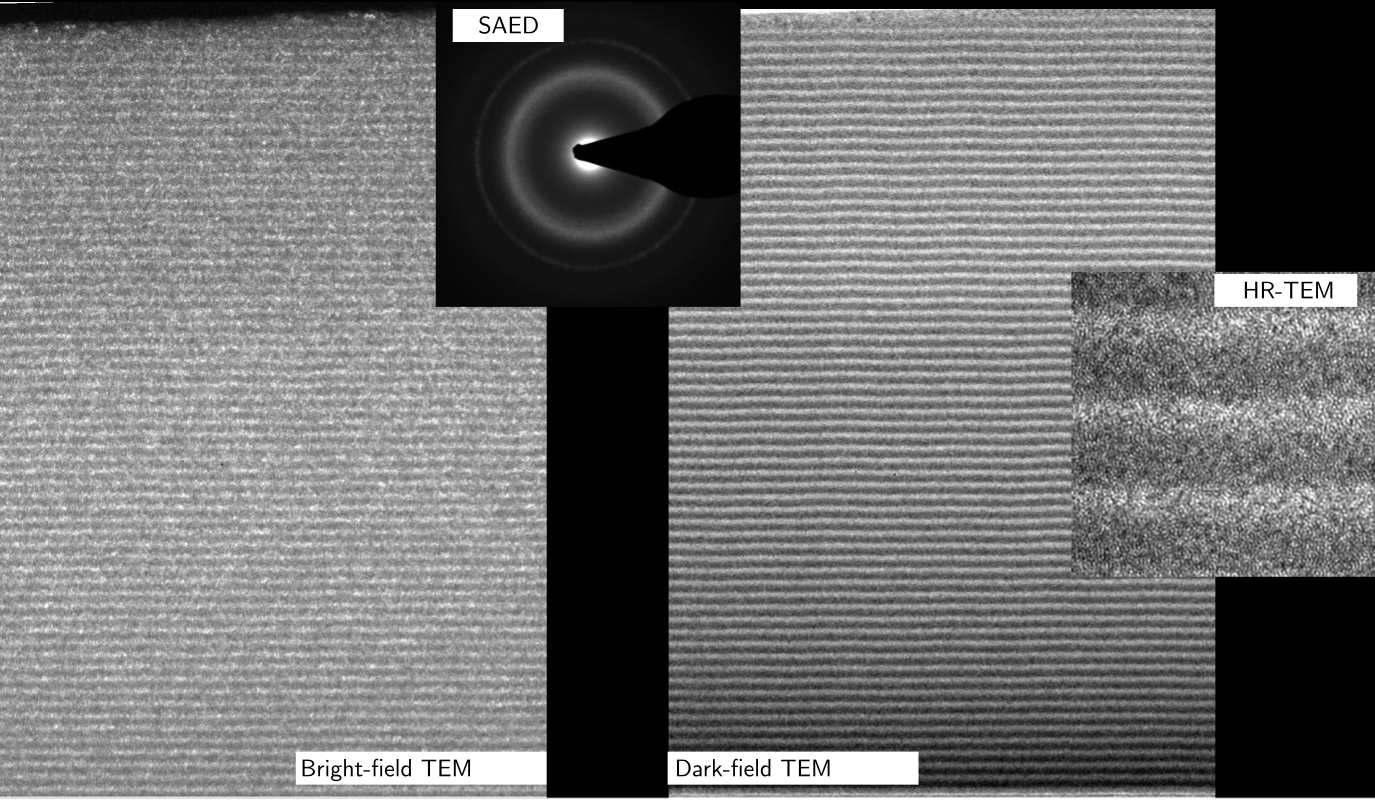
\includegraphics[width=\textwidth]{TEM.png}
	\caption{A TEM measurement of one a Ni/Ti multilayer deposited in this work. The modes of operations that have been discussed in this text are shown in the figure.}
	\label{TEMfig}
\end{figure}
\subsection{Bright-field imaging}
Bright-field (BF) imaging is often seen as the traditional imaging mode for TEM, and is therefore also known as the conventional TEM \cite{ohring}. In this mode of operation, the diffracted beam after the sample is blocked while the direct beam is allowed to pass through \cite{TEM_new}. During a practical experiment, this is achieved by placing an aperture in the back focal plane of the objective lens. The obtained contrast in the resulting image is often said to be dependent on the mass of the different elements, this is not entirely correct. Instead, the contrast is rather dependent on the atomic number Z \cite{spence2013high}, and the interference from transmitted electrons. So while heavier elements will generally absorb more, no TEM contrast will be observed for different isotopes of the same element despite a difference in mass density. Generally, as heavier elements with a higher atomic number absorb more, a multilayer with heavy/light elemental layers will respectively appear as dark/bright layers. \cite{thesis_naureen}. 
\subsection{Dark-field imaging}
With dark-field (DF) imaging, the direct beam is blocked while the diffracted beam is selected. In a practical experiment, this means that an aperture is used that blocks the transmitted beam and only allows the diffracted beam to pass \cite{TEM_new}. The resulting DF-image arises due to electron diffraction \cite{thesis_naureen}. As this mode of operation is dependent on diffraction conditions, the resulting contrast will be dependent on the formation of crystallites, making it possible to obtain local information about the crystallinity of the multilayer. 
\subsection{High Resolution Transmission Electron Microscopy}
To obtain images with an even higher magnification, high resolution transmission electron microscopy (HR-TEM) can be used. In this mode of operation, both the scattered and transmitted beams are used in order to form an interference image \cite{thesis_naureen}. This technique is based on the phase shift that the electron wave undergoes when interacting with the atoms in a sample. The interference pattern in the image plane gives rise to the contrast in HR-TEM images. Small features such as dislocations can be recorded with this technique due to the strong interaction between electrons and the atoms in the sample \cite{HRTEM}. 

\subsection{Selected Area Electron Diffraction}
Selected Area Electron Diffraction (SAED) patterns are diffraction patterns of a selected area within one sample. To obtain such a pattern, a special aperture is inserted  into the image plane to select an area of the sample. The diffraction pattern can be magnified and viewed by the TEM. Crystalline materials give rise to diffraction spots, while polycrystalline and amorphous materials give diffraction rings of varying sharpness and width, these rings can be observed as well in Figure \ref{TEMfig}. Using this mode of operation, strains and texture deviations can be found for individual grains \cite{ohring}.  